\documentclass{article}
\usepackage{amsmath}
\usepackage{enumerate}
\usepackage{fancyhdr} % Required for custom headers
\usepackage{lastpage} % Required to determine the last page for the footer
\usepackage{extramarks} % Required for headers and footers
\usepackage[usenames,dvipsnames]{color} % Required for custom colors
\usepackage{graphicx} % Required to insert images
\usepackage[tight,footnotesize]{subfigure} % Required for subfig
\usepackage{caption} % Required for subfig
\usepackage{hyperref} % Required for url
\usepackage{listings} % Required for insertion of code
\usepackage{courier} % Required for the courier font
\usepackage{lipsum} % Used for inserting dummy 'Lorem ipsum' text into the template
\topmargin=-0.45in
\evensidemargin=0in
\oddsidemargin=0in
\textwidth=6.5in
\textheight=9.0in
\headsep=0.25in
\linespread{1.1} % Line spacing
\pagestyle{fancy}
\lhead{\hmwkAuthorName} % Top left header
% \chead{\hmwkClass\ (\hmwkClassInstructor\ \hmwkClassTime): \hmwkTitle} % Top center head
\chead{\hmwkClass\ : \hmwkTitle} % Top center head
\rhead{\firstxmark} % Top right header
\lfoot{\lastxmark} % Bottom left footer
\cfoot{} % Bottom center footer
\rfoot{Page\ \thepage\ of\ \protect\pageref{LastPage}} % Bottom right footer
\renewcommand\headrulewidth{0.4pt} % Size of the header rule
\renewcommand\footrulewidth{0.4pt} % Size of the footer rule
\setlength\parindent{0pt} % Removes all indentation from paragraphs

% Define floor and ceiling
\def\lc{\left\lceil}   
\def\rc{\right\rceil}
\def\lf{\left\lfloor}   
\def\rf{\right\rfloor}

% table
\usepackage[table,xcdraw]{xcolor}
\usepackage{floatrow}
\newfloatcommand{capbtabbox}{table}[][\FBwidth]

% draw tree
\usepackage{tikz, tikz-qtree}
\usetikzlibrary{arrows,snakes,backgrounds,patterns,matrix,shapes,fit,calc,positioning,trees}
\tikzset{main node/.style={circle,fill=blue!20,draw,minimum size=1cm,inner sep=0pt},}

% Set your language 
%\lstset{language=Java}
\definecolor{codegreen}{rgb}{0,0.6,0}
\definecolor{codegray}{rgb}{0.5,0.5,0.5}
\definecolor{codepurple}{rgb}{0.58,0,0.82}
\definecolor{backcolour}{rgb}{0.95,0.95,0.92}
 
\lstdefinestyle{mystyle}{
    backgroundcolor=\color{backcolour},   
    commentstyle=\color{codegreen},
    keywordstyle=\color{magenta},
    numberstyle=\tiny\color{codegray},
    stringstyle=\color{codepurple},
    basicstyle=\footnotesize,
    breakatwhitespace=false,         
    breaklines=true,                 
    captionpos=b,                    
    keepspaces=true,                 
    numbers=left,                    
    numbersep=8pt,                  
    showspaces=false,                
    showstringspaces=false,
    showtabs=false,                  
    tabsize=2
}
\lstset{style=mystyle}

% Header and footer for when a page split occurs within a problem environment
\newcommand{\enterProblemHeader}[1]{
\nobreak\extramarks{#1}{#1 continued on next page\ldots}\nobreak
\nobreak\extramarks{#1 (continued)}{#1 continued on next page\ldots}\nobreak
}

% Header and footer for when a page split occurs between problem environments
\newcommand{\exitProblemHeader}[1]{
\nobreak\extramarks{#1 (continued)}{#1 continued on next page\ldots}\nobreak
\nobreak\extramarks{#1}{}\nobreak
}

\setcounter{secnumdepth}{0} % Removes default section numbers
\newcounter{homeworkProblemCounter} % Creates a counter to keep track of the number of problems

\newcommand{\homeworkProblemName}{}
\newenvironment{homeworkProblem}[1][Problem \arabic{homeworkProblemCounter}]{ % Makes a new environment called homeworkProblem which takes 1 argument (custom name) but the default is "Problem #"
\stepcounter{homeworkProblemCounter} % Increase counter for number of problems
\renewcommand{\homeworkProblemName}{#1} % Assign \homeworkProblemName the name of the problem
\section{\homeworkProblemName} % Make a section in the document with the custom problem count
\enterProblemHeader{\homeworkProblemName} % Header and footer within the environment
}{
\exitProblemHeader{\homeworkProblemName} % Header and footer after the environment
}

\newcommand{\problemAnswer}[1]{ % Defines the problem answer command with the content as the only argument
\noindent\framebox[\columnwidth][c]{\begin{minipage}{0.98\columnwidth}#1\end{minipage}} % Makes the box around the problem answer and puts the content inside
}

\newcommand{\homeworkSectionName}{}
\newenvironment{homeworkSection}[1]{ % New environment for sections within homework problems, takes 1 argument - the name of the section
\renewcommand{\homeworkSectionName}{#1} % Assign \homeworkSectionName to the name of the section from the environment argument
\subsection{\homeworkSectionName} % Make a subsection with the custom name of the subsection
\enterProblemHeader{\homeworkProblemName\ [\homeworkSectionName]} % Header and footer within the environment
}{
\enterProblemHeader{\homeworkProblemName} % Header and footer after the environment
}

\newlength{\tabcont}

\newcommand{\tab}[1]{%
\settowidth{\tabcont}{#1}%
\ifthenelse{\lengthtest{\tabcont < .25\linewidth}}%
{\makebox[.25\linewidth][l]{#1}\ignorespaces}%
{\makebox[.5\linewidth][l]{\color{red} #1}\ignorespaces}%
}%
%----------------------------------------------------------------------------------------------
%	NAME AND CLASS SECTION
%----------------------------------------------------------------------------------------------

\newcommand{\hmwkTitle}{Homework\ \#10} % Assignment title
\newcommand{\hmwkDueDate}{Monday,\ January\ 1,\ 2012} % Due date
\newcommand{\hmwkClass}{Fundamental Algorithms} % Course/class
\newcommand{\hmwkClassTime}{} % Class/lecture time
\newcommand{\hmwkClassInstructor}{Prof. Joel Spencer} % Teacher/lecturer
\newcommand{\hmwkAuthorName}{Songxiao Zhang, N10224459, {\tt 72}} % Your name

%----------------------------------------------------------------------------------------------
%	TITLE PAGE
%----------------------------------------------------------------------------------------------

\title{
\textmd{\textbf{\hmwkClass:\ \hmwkTitle}}\\
}
\author{\textbf{\hmwkAuthorName}}

\begin{document}

\maketitle

%----------------------------------------------------------------------------------------------
%	PROBLEM 1
%----------------------------------------------------------------------------------------------
\begin{homeworkProblem}
Suppose the edge $\{x,y\}_0$ in $T$ and $w\{x,y\}_1$ not in $T$. Now $w\{x,y\}_1$ is reduced to
$w\{x,y\}_2$. By definition, 
$$w(T) = \sum\limits_{(u,v) \in T} w(u,v)$$    

$\{x,y\}_1$ was not in $T$ because $w\{x,y\}_1$ was larger than $w\{x,y\}_0$. Now
$\{x,y\}_1$ in $T$ replaces $\{x,y\}_0$ now in $T$. The MST is changed to 
$T - \{x,y\}_0 \cup \{x,y\}_1$. Its weight is now $w(T) - w\{x,y\}_0 + w\{x,y\}_1$. 
\end{homeworkProblem}

%----------------------------------------------------------------------------------------------
%	PROBLEM 2
%----------------------------------------------------------------------------------------------
\begin{homeworkProblem}

\begin{enumerate}[(a)]
    \item Kruskal is a minimum-spanning-tree algorithm. $n-1$ edges and $n$ vertices can form
          a acyclic spanning tree, since it requires at least $n$ edges to form a cycle, and 
          $k$ cycles requires $(n-1+k)$ edges. \\
          At each step, only the edge with the minimum weight connecting two trees 
          would be added to the forest, which makes Kruskal a greedy algorithm. No more edges
          added. The total weight of the tree (or forest if not all connected) would be the 
          minimal cost connecting all vertices. 
          
    \item Sorting edge would be avoided in Kruskal. \\
          $O(n)$ - inserting all vertices to hashset    \\
          $O(1)$ - search edge $\{u, v\}$ in hashset for $n$ vertices, 
                    where $u$ and $v$ are not in the same tree.  \\
          $O(\lg n)$ - union edge $\{u, v\}$ in hashset for $n$ vertices, ,
                    where $u$ and $v$ are not in the same tree. \\
          Since $|n|^2 > |m| \geq |n| - 1$, the total running time would be $O(n\lg n)$. 
          
    \item Union operation now increases to $O(n)$ for $n=2k$ vertices in total. 
          The running time is $O(n^2)$ now. The union operation appends the roots of all 
          small trees to the root of the largest tree. 
          For example, the edge list is 
          $\{u, v\} \in \{(1,2), (2,3), ..., (k-1,k), (k+1,1), (k+2,1), ..., (n,1) \}$. 
          The graph would look like a broom, $(k+1) to n$ vertices point to vertex $k$ and 
          $1->2->...->k$ where $k$ is the root. \\
          In total, {\em Dumb Kruskal} takes 
          $\sum\limits_{i=1}^{\frac{n}{2}}i + \frac{n}{2}\frac{n}{2}
          = \frac{(\frac{n}{2} + 1)\frac{n}{2}}{2} + \frac{n^2}{4} = \Theta(n^2)$. 
          
\end{enumerate}

\end{homeworkProblem}

%----------------------------------------------------------------------------------------------
%	PROBLEM 3
%----------------------------------------------------------------------------------------------
\begin{homeworkProblem}
\begin{enumerate}[(a)]
    \item Since the weight of the edges increases as processed, 
          at each step, a vertex is appended to the list and the root remains the first element.\\
          Step 1: Processing $\{1, 2\},\ SIZE(x) = SIZE(x) + SIZE(y) = 1 + 1 = 2,\ \pi(2) = 1$ \\
          Step 2: Processing $\{2, 3\},\ SIZE(x) = SIZE(x) + SIZE(y) = 2 + 1 = 3,\ \pi(3) = 1$ \\
          Step 3: Processing $\{3, 4\},\ SIZE(x) = SIZE(x) + SIZE(y) = 3 + 1 = 4,\ \pi(4) = 1$ \\
          $\ldots$ \\
          Step 73: Processing $\{72, 73\},\ SIZE(x) = SIZE(x) + SIZE(y) = 72 + 1 = 73,\ \pi(73) = 1$    \\
        %   $\ldots$ \\
        %   Step 100: Processing $\{99, 100\},\ SIZE(x) = SIZE(x) + SIZE(y) = 99 + 1 = 100,\ \pi(100) = 1$   \\
          
    \item Traversing $n$ vertices back to the root of the forest takes $O(n)$. So in total, 
          $O(\sum\limits_{i=1}^{n}i) = O(n^2)$. 
\end{enumerate}

\end{homeworkProblem}

%----------------------------------------------------------------------------------------------
%	PROBLEM 4
%----------------------------------------------------------------------------------------------
\begin{homeworkProblem}
\begin{enumerate}[(a)]
    \item The weight function $(j-i)^2$ makes the greedy probing function always found the 
          minimum weight edge crossing is $(i, j)$ where $j = i + 1$, 
          since all $j$ that $j \leq i$ already in the
          same comp and for $j > i + 1$ has a larger weight. \\
          These 73 elements formed a linear list 
          $\{ \{1, 2\}, \{2, 3\}, \{3, 4\}, \ldots, \{72, 73\} \}$. And edge list would be\\
            \begin{table}[h]
            \begin{tabular}{lll}
            Vertex & Edge  & Weight  \\
              2    &  1-2   & 1      \\
              3    &  2-3   & 1      \\
              4    &  3-4   & 1      \\
                   &  ...   &        \\
              73   &  72-73 & 1     
            \end{tabular}
            \end{table}

    \item The $\pi$ is different in Prim's than the Kruskal's. For $\pi(x) = y$, in Prim's, 
          $y$ is the end point of the edge in process, while in Kruskal, $y$ is the root of the
          current forest. \\
          $\pi[84] = 73$ and in the list, the closest one to 84 is 73, so 
          $key[84] = min(w(84, 1:73)) = min\{(84-1)^2, (84-2)^2,..., (84-73)^2) = (84 - 73)^2 = 121$.
\end{enumerate}
\end{homeworkProblem}



% \begin{lstlisting}[frame=single]
% \end{lstlisting}

% \begin{enumerate}[a.]
%     \item 
        %   
% \end{enumerate}

% \begin{figure}[h!]
%     \centering
%     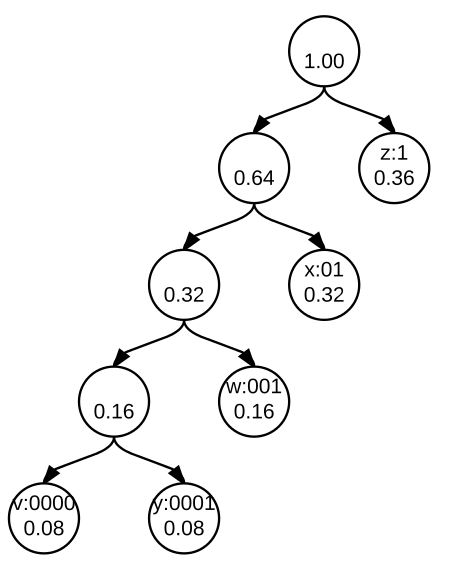
\includegraphics[scale=0.4]{hw8/2.png}
%     \caption{}
%     \label{fig:forz}
% \end{figure} 

% Figure~\ref{fig:tree} on Page~\pageref{fig:tree}.
% \begin{figure}[h!]
%     \centering
%     \subfigure[]{\label{}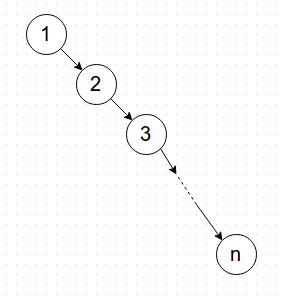
\includegraphics[scale=0.4]{hw6/51.png}}
%     \subfigure[]{\label{}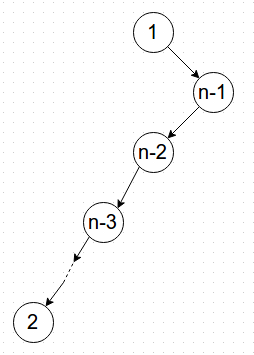
\includegraphics[scale=0.4]{hw6/52.png}}
%     \caption{}
%     \label{fig:tree}
% \end{figure} 

% \begin{tikzpicture}
%   [scale=.6,auto=left,every node/.style={circle,fill=blue!20}]
%   \node (n1) at (6, 6) {1};
%   \node (n2) at (4,3)  {2};
%   \node (n3) at (2,0) {3};
%   \foreach \from/\to in {n1/n2,n2/n3}
%     \draw (\from) -- (\to);
% \end{tikzpicture}

% \begin{tikzpicture}[
% >=stealth', semithick, node distance=1cm, level distance=15mm, 
%     level/.style={sibling distance=30mm/#1},
%     round/.style = {draw, circle, fill=blue!20, scale=0.8,minimum height=1cm},
%     every node/.style={circle, draw, fill=none, anchor=north},
% ]
% \node (tree 1) [draw=none, rectangle] {\tikz{%
% \node (tree 1) [round] {Q(1,16)}
%     child{ node[round] {S(2,7)} }
% }};
% \node (tree 2) [draw=none, rectangle, right=of tree 1] {\tikz{%
% \node (tree 2) [round] {R(17,20)}
% }};
% \end{tikzpicture}

\end{document}